\documentclass[a4paper, 12pt]{article}


\usepackage[czech]{babel}
\usepackage[utf8]{inputenc}


\usepackage[top=2.5cm,bottom=2.5cm,left=3.5cm,right=2.5cm]{geometry}
\usepackage{times}
\usepackage{graphicx}
\usepackage[dvipsnames]{xcolor} % for colored text
\usepackage[colorlinks=true, allcolors=RoyalBlue]{hyperref}
\usepackage{tocloft} % Table of contents
\usepackage{multicol} % Multiple columns
\usepackage{wrapfig}
\usepackage{index}
\usepackage{courier} % Sets font for listing as Courier.
\usepackage{listings, xcolor}
\usepackage{tcolorbox}
\usepackage{subfig}
\usepackage{setspace}
\usepackage{titlesec}
\usepackage{todonotes}
\usepackage{csquotes}
\usepackage{filecontents} % data or code snippets from external sources
\usepackage{ragged2e}



% Sections on new page
\newif\ifclearpageenabled
\clearpageenabledtrue % Set the variable to true by default
\AddToHook{cmd/section/before}{
    % Check if \clearpageenabled is true
    \ifclearpageenabled
        \clearpage % Execute \clearpage if true
    \fi
}




% Ukázky kódu
\renewcommand\lstlistlistingname{Seznam ukázek kódu}
\renewcommand\lstlistingname{Ukázka}
\definecolor{backcolour}{rgb}{0.95,0.95,0.92}
\lstdefinestyle{Python}{
    language=Python,
    basicstyle=\scriptsize\fontfamily{lmtt}\selectfont,
    backgroundcolor=\color{backcolour},
    keywordstyle=\color{blue},
    commentstyle=\color{green!40!black},
    stringstyle=\color{RedViolet},
    showstringspaces=false,
    breaklines=true,
    breakatwhitespace=true,
    tabsize=4,
    numbers=left,
    numberstyle=\tiny\color{gray},
    frame=single,
    columns=fullflexible,
    % rulecolor = \color{black}, %% set frame color to avoid being affected by text color
}

\lstdefinelanguage{JavaScript}{
  keywords={typeof, new, true, false, catch, function, return, null, catch, switch, var, if, in, while, do, else, case, break},
  keywordstyle=\color{blue}\bfseries,
  ndkeywords={class, export, boolean, throw, implements, import, this},
  ndkeywordstyle=\color{darkgray}\bfseries,
  identifierstyle=\color{black},
  sensitive=false,
  comment=[l]{//},
  morecomment=[s]{/*}{*/},
  commentstyle=\color{purple}\ttfamily,
  stringstyle=\color{red}\ttfamily,
  morestring=[b]',
  morestring=[b]"
}

\lstdefinestyle{JavaScript}{
    language=JavaScript,
    basicstyle=\scriptsize\fontfamily{lmtt}\selectfont,
    backgroundcolor=\color{backcolour},
    keywordstyle=\color{blue},
    commentstyle=\color{green!40!black},
    stringstyle=\color{RedViolet},
    showstringspaces=false,
    breaklines=true,
    breakatwhitespace=true,
    tabsize=4,
    numbers=left,
    numberstyle=\tiny\color{gray},
    frame=single,
    columns=fullflexible,
    % rulecolor = \color{black}, %% set frame color to avoid being affected by text color
}


\lstdefinelanguage{XML_SYNTAX}{%
    alsoletter=-,
    morestring=[b]",stringstyle=\color[rgb]{0,0,1},
    moredelim=*[s][{\color[rgb]{0.75,0,0}}]{<}{>},
    moredelim=[s][{\color[rgb]{0,0,0}}]{<!--}{-->},
    moredelim=[s][{\color[rgb]{0,0.75,0}}]{\ }{=},
    moredelim=[s][{\color[rgb]{0,0.75,0}}]{\    }{=} % here there is \tab
}

\lstdefinestyle{HTML}{
    % Basic design
    backgroundcolor=\color{backcolour},
    basicstyle=\scriptsize\fontfamily{lmtt}\selectfont,
    breaklines=true,
    frame=l,
    tabsize=4,    
    breakatwhitespace=true,
    numbers=left,    
    numberstyle=\tiny\color{gray},
    frame=single,
    numberfirstline=true,
    % HTML formatting
    language=XML_SYNTAX,
}

\lstdefinelanguage{CSS}{
  keywords={background-color, height, width, border, radius, animation, opacity, position, z, index, background, color, transform, left, right, content, top, margin, padding, overflow, backdrop, filter, box, shadow, webkit, transition},
  keywordstyle=\color{blue}\bfseries,
  ndkeywords={ ease, in, out, infinite, both, alternate, var, px, rem, s},
  ndkeywordstyle=\color{green!50!black}\bfseries,
  identifierstyle=\color{brown}\bfseries,
  sensitive=false,
  comment=[l]{/*},
  morecomment=[s]{/*}{*/},
  commentstyle=\color{purple}\ttfamily,
  stringstyle=\color{red}\ttfamily,
  morestring=[b]',
  morestring=[b]"
}

\lstdefinestyle{CSS}{
    language=CSS,
    basicstyle=\scriptsize\fontfamily{lmtt}\selectfont,
    backgroundcolor=\color{backcolour},
    keywordstyle=\color{blue},
    commentstyle=\color{green!40!black},
    stringstyle=\color{RedViolet},
    showstringspaces=false,
    breaklines=true,
    breakatwhitespace=true,
    tabsize=4,
    numbers=left,
    numberstyle=\tiny\color{gray},
    frame=single,
    columns=fullflexible,
    % rulecolor = \color{black}, %% set frame color to avoid being affected by text color
}



% List of figures
\renewcommand{\cftloftitlefont}{\LARGE\bfseries}
\renewcommand\cftfigfont{\small}
\renewcommand\cftfigpagefont{\small}


% Bibliography
\usepackage[natbib=true,
    style=numeric,
    sorting=none]{biblatex}
\addbibresource{ref.bib}
% Define a command to set the font size for the bibliography entries
\newcommand{\setbibfont}{\small} 
\AtBeginBibliography{\setbibfont}



%% Section font format¨
\titleformat*{\section}{\LARGE\bfseries}
\titleformat*{\subsection}{\Large\bfseries}
\titleformat*{\subsubsection}{\large\bfseries}
\titleformat*{\paragraph}{\large\bfseries}
\titleformat*{\subparagraph}{\large\bfseries}

\emergencystretch=3em
\setstretch{1.15}
\parindent=0pt % Zrušení odsazení prvního řádku odstavce
\parskip=12pt % Mezera mezi odstavci (12 bodů)
%\hyphenpenalty=10000\exhyphenpenalty=10000 %žádné pomlčky na konci
\setlength {\marginparwidth }{2cm} 


\begin{document}



\pagenumbering{gobble} %%no page number

\renewcommand{\cftsecleader}{\cftdotfill{\cftdotsep}}
\title{\textbf{Maturitní práce}}

\author{} %fix alert
\maketitle

\centerline{\Large {\textbf{ Gymnázium, Praha 6, Arabská 14}} \par}
\centerline{ \large    Arabská 14, Praha 6, 160 00 \par} 
\begin{figure}[hp]
    \centering
    
\includegraphics[scale = 0.5]{Images/GA_logo.png}
    
\end{figure}

\vfill
\begin{flushleft}
\textbf{Předmět:} Programování\newline
\textbf{Téma:} Tempora - Stránka pro tvorbu interaktivních časových os  \newline
\newline
\textbf{Autor:} \author{\textit{Jiří Petřík}} \newline
\textbf{Třída:} 4.E  \newline
\textbf{Vyučující:} Mgr. Jan Lána \newline
\textbf{Tř. vyučující:} Mgr. Blanka Hniličková

\end{flushleft}
% Turn off \clearpage for specific pages
\clearpageenabledfalse % Disable \clearpage
\newpage


\mbox{}
\vfill
\begin{Large}
\section*{Čestné prohlášení:}
\end{Large}
\par Prohlašujeme, že jsem jediným autorem tohoto projektu, všechny citace jsou řádně označené a všechna použitá literatura a další zdroje jsou v práci uvedeny. 
\par Tímto dle zákona 121/2000 Sb. (tzv. Autorský zákon) ve znění pozdějších předpisů uděluji bezúplatně škole Gymnázium, Praha 6, Arabská 14 oprávnění k výkonu práva na rozmnožování díla (§ 13) a práva na sdělování díla veřejnosti (§ 18) na dobu časově neomezenou a bez omezení územního rozsahu. 

\vspace{40pt}
\noindent
V Praze dne …………………… \hspace{20pt} …………………… \\


\clearpageenabledtrue % Re-enable \clearpage for subsequent pages
%\renewcommand{\cftsecleader}{\cftdotfill{\cftdotsep}}
\begin{center}
    \textbf{\large STŘEDOŠKOLSKÁ ODBORNÁ ČINNOST} \\[1cm]
    \textbf{Obor č. 12. Tvorba učebních pomůcek, didaktická technologie}
    
\end{center}

\vfill

\begin{center}
    \textbf{\Large {Tempora - Stránka pro tvorbu interaktivních časových os}}
\end{center}

\vfill

\begin{tabular}{p{0.7\textwidth} p{0.3\textwidth}}
    \textbf{{Jiří Petřík}} \\[0.2cm]
    \textbf{Pražský kraj} & 
    \textbf{{Praha 2025}}
\end{tabular}


%% Turn off \clearpage for specific pages
\clearpageenabledfalse % Disable \clearpage
\newpage

\begin{center}
    \textbf{\large STŘEDOŠKOLSKÁ ODBORNÁ ČINNOST} \\[1cm]
    \textbf{Obor č. 12. Tvorba učebních pomůcek, didaktická technologie}
    
\end{center}

\vfill

\begin{center}
     \textbf{\Large {Tempora - Stránka pro tvorbu interaktivních časových os}}
    \newline
     \textbf{\Large {Tempora - Webside for creation of interactive timelines}}
\end{center}

\vfill

\begin{flushleft}
    \textbf{Autor:} {Jiří Petřík} \\[0.2cm]
    \textbf{Škola:} {Gymnázium, Praha 6, Arabská 14, Arabská 682/14,
    160 00, Praha 6 - Vokovice } \\[0.2cm]
    \textbf{Kraj:} Pražský kraj \\[0.2cm] 
    \textbf{Konzultant:} {Mgr. Jan Lána}
\end{flushleft}

\vspace{1cm}

\begin{flushleft}
    \textcolor{black}{Praha 2025}
\end{flushleft}

%% Turn off \clearpage for specific pages
\clearpageenabledfalse % Disable \clearpage
\newpage

\begin{Large}
\section*{Prohlášení}
\end{Large}



Prohlašuji, že jsem svou práci SOČ vypracoval samostatně a použil jsem pouze prameny a literaturu uvedené v seznamu bibliografických záznamů.

Prohlašuji, že tištěná verze a elektronická verze soutěžní práce SOČ jsou shodné. 

Nemám závažný důvod proti zpřístupňování této práce v souladu se zákonem č. 121/2000 Sb., o právu autorském, o právech souvisejících s právem autorským a o změně některých zákonů (autorský zákon) ve znění pozdějších předpisů. 

\vspace{40pt}

V Praze dne ……………… \hspace{20pt} …………………… \\


\clearpageenabledtrue % Re-enable \clearpage for subsequent pages
\clearpageenabledfalse % Disable \clearpage
\newpage

\section*{Poděkování}

Chtěl bych poděkovat Vítězslavu Procházkovi za pomoc s výběrem technologií a přínosné konzultace a Ing. Ivu Petříkovi za zpětnou vazbu a návrhy na zlepšení projektu. 

\clearpageenabledtrue

\clearpageenabledfalse % Disable \clearpage
\newpage
\section*{Anotace}

Ve své práci SOČ jsem se zabýval vývojem webové stránky sloužící jako nástroj pro vytváření a vizualizaci interaktivních časových os. Cílem práce bylo umožnit uživatelům tvorbu, procházení a sdílení časových os s možností jejich rozkliknutí pro podrobnější informace o jednotlivých obdobích a autorech. Tyto osy se vyznačují důrazem na zasazení událostí do historického kontextu a umožňují srovnání dvou tématicky odlišných období.

Projekt byl naprogramován s využitím open-source frameworku Nuxt.js a databázové platformy Supabase.

\section*{Klíčová slova}
Časová osa; webová stránka; učební pomůcka; historický kontext

\vspace{40pt}

\section*{Annotation}
In my SPA work, I have been developing a website used as a tool for creating and visualizing interactive timelines. The aim of the work was to allow users to create, browse, and share timelines with the ability to click through for more detailed information about each period and author. These timelines are specific in that they emphasize placing events in a historical context and provide the ability to compare two thematically distinct periods.

The project was programmed using the open-source framework Nuxt.js and the database platform Supabase.

\section*{Keywords}
Timeline; website; learning tool; historical context


\clearpageenabledtrue 


\newpage
\pagenumbering{arabic} % start numbering pages
% \linespread{0.9}\selectfont
\tableofcontents
% \linespread{1.5}\selectfont



\section{Úvod}

Orientace v dějinách je často komplikovaná, zejména pokud se snažíme pochopit souvislosti mezi různými historickými událostmi, osobnostmi a směry. Setkáváme se s velkým objemem historických informací, letopočtů, významných událostí, konfliktů, ale i nových objevů a vynálezů, a proto je velmi obtížné získat ucelený přehled o zasazení jednotlivých událostí do dějin.
Tradiční přístupy k výuce historie často pracují s oddělenými časovými liniemi napříč několika studijními předměty, což ztěžuje porovnání událostí probíhajících ve stejném období, ale v odlišných kontextech. V mém projektu se proto snažím vytvořit nástroj, který by tento problém pomohl uživatelům vyřešit.

Jméno Tempora pochází z množného čísla latinského slova tempus = čas. Logo projektu jsem sám vytvořil – znázorňuje jednotlivé úseky na časové ose a používám ho jako favicon projektu \cite{Favicon}.

\subsection{Cíl projektu}

Cílem projektu Tempora je poskytnout uživatelům nástroj pro tvorbu a vizualizaci interaktivních časových os, který umožní jednoduché porovnávání různých témat v daném období, jejich zasazení do historického kontextu a přehledné zobrazení dat. Důležitou součástí projektu je vytvořit tuto osu interaktivní a uživatelsky příjemnou, s možností rozkliknutí jednotlivých období, ke kterým jsou vytvořeny podrobnější popisy, vysvětlivky nebo případně odkazy na další informace.



\vspace{2cm}

\begin{figure}[h]
    \centering
    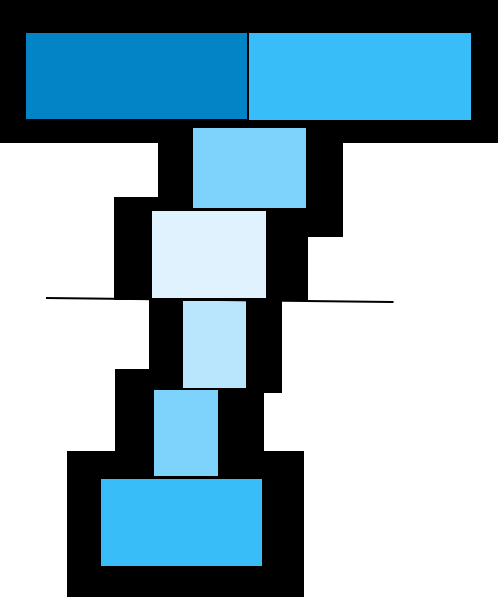
\includegraphics[width=0.25\linewidth]{Images/TemporaLogo_big.png}
    \caption{Logo Tempora}
    \label{fig:logo}
\end{figure}
\section{Použité technologie}

Projekt je postaven na frameworku Nuxt \cite{NUXT}, který je určený pro tvorbu webových aplikací a stránek pomocí Vue.js \cite{Vue.js}. Nuxt byl vybrán díky své flexibilitě a funkcím, jako je automatické routování stránek, asynchronní data, lazy-loading, automatická importace modulů \cite{NuxtImport-Fix} a široký ekosystém modulů a podporovaných knihoven.

O databázi se stará služba Supabase \cite{Supabase}, která využívá PostgreSQL (více v kapitole \ref{Backend} \textit{Backend}).

Pro design webové stránky jsem použil Tailwind CSS \cite{Tailwind-CSS}, který se řídí principem utility-first, používá intuitivní syntaxi a konzistentní barvy \cite{Colors-tailwind, Hex-Color-tailwind}.
Celý kód mého projektu jsem průběžně zálohoval pomocí Gitu na službu GitHub do repozitáře \href{https://github.com/gyarab/2024-4e-petrik-Tempora}{Tempora} organizace gyarab \cite{gyarab-github}.

\section{Frontend}

Webová aplikace je z velké části napsána ve Vue.js. Tato JavaScriptová knihovna pro tvorbu uživatelských rozhraní využívá komponentový přístup, který umožňuje rozdělit uživatelské rozhraní do logických a znovupoužitelných částí. To pomáhá udržet dobrou organizaci a architekturu projektu.

\subsection{Vlastní komponenty}
Jak již bylo zmíněno, Nuxt a Vue.js jsou založeny na znovupoužívání komponent pro zachování jednoduchosti na hlavních stránkách. Vytvořil jsem devět komponent, z nichž nejdůležitější je \textbf{\textit{TimelineComp.vue}}. Tento komponent v sobě ukrývá veškeré prvky týkající se přímo časové osy, jako jsou například CSS styly nebo ovládání osy.

Na stránce, kde se nachází časová osa, je také postranní menu vytvořené v \textbf{\textit{SidebarComp.vue}}. Obsahuje uživatelské funkce, jako je přepínání barevného režimu časové osy nebo sdílení odkazu na danou osu.

Dále existují komponenty, které se přepínají podle potřeby. Například když uživatel klikne na událost, zobrazí se \textbf{\textit{ItemInfoComp.vue}}, který poskytne informace. Pokud je však uživatel v editačním režimu, objeví se \textbf{\textit{ItemEditComp.vue}}, který umožní změnit informace o události. Podobným způsobem funguje i \textbf{\textit{InfoComp.vue}}, zobrazující informace o časové ose, a \textbf{\textit{SettingsComp.vue}}, který umožňuje upravovat hodnoty časové osy. Komponent \textbf{\textit{CreateTimeline.vue}} se zobrazí pouze tehdy, když chce uživatel vytvořit novou časovou osu, a slouží k zadání potřebných informací.

Komponent \textbf{\textit{LineCard.vue}} slouží jako šablona karty jednotlivých časových os, do níž se vkládají informace o autorovi nebo letech, které osa pokrývá.

Poslední komponent je \textbf{\textit{QuillEditor.vue}} z knihovny Quill \cite{Quill-lib}, který umožňuje uživateli používat různé textové prvky.

\newpage

\subsection{Rozdělení stránek}
V Nuxt jsou stránky definovány v adresáři \textit{pages/}, kde název .vue souboru a složky/složek, ve kterých se nachází, určuje jeho URL adresu. Názvy souborů mohou být buď statické (např. pages/about, pages/login), nebo dynamické, které pracují s proměnnými, přičemž jejich jméno je v hranatých závorkách (např. pages/[id]: pokud zadáme adresu \texttt{lines/6}, zobrazí se stránka „[id].vue“ složky lines s proměnnou 6, se kterou lze dále pracovat pomocí Vue Routeru \cite{NUXT}). Základní stránka každé složky se vždy jmenuje \textit{index.vue} a její název se nezobrazuje v URL. Nuxt také ve výchozím nastavení implementuje plně přizpůsobitelnou stránku \textit{error.vue}, na kterou jste přesměrováni, pokud nastane nějaká fatální chyba.

Strukturu mé webové stránky lze rozdělit do tří vrstev. První vrstva zahrnuje přihlášení, registraci, domovskou stránku uživatele a stránku „O projektu“. Ve druhé vrstvě se nachází „Přehled časových os“ (\textit{lines/index}), kde mohou uživatelé vyhledávat vytvořené osy, zobrazit si o nich informace, aniž by museli osu načíst, nebo vytvořit nové časové osy. Poslední, třetí vrstva obsahuje samotnou časovou osu (\textit{lines/id/index}) a podrobnosti o jednotlivých událostech (\textit{lines/id/content}).

Funkci dynamických stránek jsem ve svém projektu použil dvakrát – při výběru ID dané osy a při podrobném zobrazení údajů o události. Pokud by tedy uživatel chtěl zobrazit podrobnosti o události 17 v ose s ID 123456, výsledná URL adresa bude \texttt{/lines/123456/17}.


\begin{figure}[h]
    \centering
    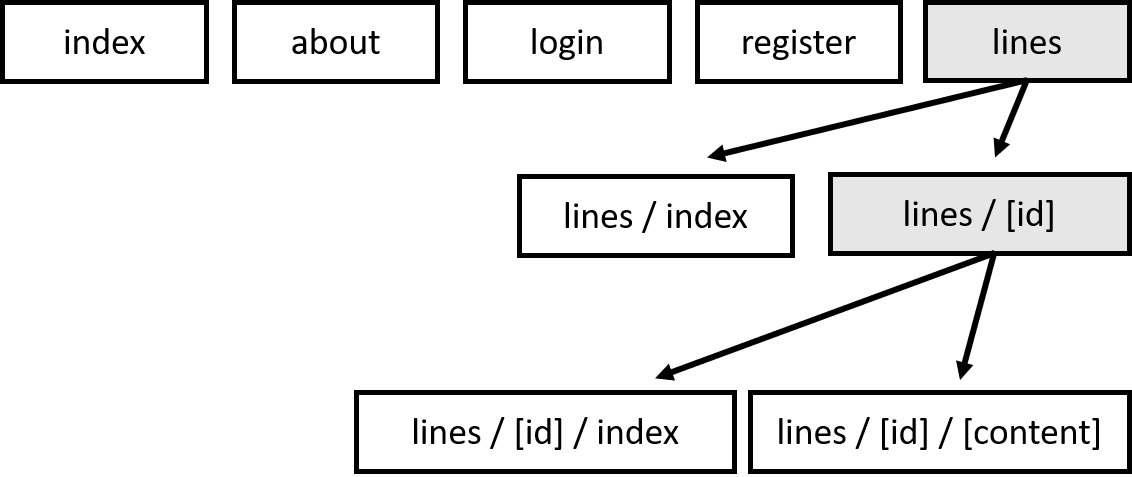
\includegraphics[width=0.8\linewidth]{Images/Tempora_pages.png}
    \caption{Rozdělení stránek ( [ ] = dynamická stránka, šedá = složka)}
    \label{fig:pages}
\end{figure}
Nuxt také používá funkci lazy-loading, která přednačítá stránky dosažitelné ze stránky aktuální pomocí speciálního odkazu NuxtLink. Tento přístup výrazně zrychluje načítání, například při rozkliknutí podrobností o události ze stránky s časovou osou.

\subsection{Moduly a knihovny}

Nuxt s Vue.js nabízí velkou škálu různých modulů, které přidávají novou funkcionalitu a rozšiřují možnosti. Jelikož jsem nikdy předtím s ekosystémem Nuxt nepracoval, na některá z těchto vylepšení jsem přicházel postupně v průběhu projektu \cite{libraries-on-EVERY-project, Nuxt3-Crash-Course}.

Jeden z nejužitečnějších modulů je NuxtUI \cite{NUXT-UI}, který přidává nejrůznější frontendové komponenty, jako jsou např. modal a toggle, ale zároveň poskytuje i vylepšené základní komponenty, například UButton, u kterého lze nastavit parametry pro ikonu, barvu či velikost. NuxtUI přidává také animovanou postranní lištu, ale tu jsem vytvořil ještě před instalací tohoto rozšíření \cite{sidebar}.

Jednou z funkcí mé aplikace je, že v zobrazení detailu můžete vidět názvy sekcí, které následují a předcházejí zobrazené sekci, což pomáhá s orientací v období. Toto zajišťuje state management framework Pinia \cite{Pinia-store}.

\subsection{Modul a komponent časové osy} \label{Komponent časové osy}

Nejdůležitější knihovna, která byla použita, je Vue Timeline Chart \cite{Vue-timeline-chart}. Hlavním důvodem, proč jsem si vybral právě tuto knihovnu, byla její flexibilita a dobře zpracovaná dokumentace. Základem této osy jsou řádky (timelineGroup) a události (timelineItem). Události mají několik údajů, jako je jméno, unikátní ID, start a end, udávané v milisekundách Unixového času (od 1. ledna 1970, 00:00:00 UTC – epoch). Základní časová osa není nijak komplikovaná, ale pokud chceme změnit její vzhled, musíme správně použít CSS a přepsat výchozí styly.

Mojí vizí bylo vytvořit dvě strany uprostřed rozdělené časovou osou, přičemž každá strana bude mít čtyři řádky s velikostí podle jejich důležitosti. Nahoře a dole bude kontext k období, dále „Hlavní skupina“, která obsahuje nadpis období, „Vedlejší skupina“, obsahující převážně autory z daného období, a nakonec „Detail skupina“, která slouží k zobrazení dalších informací, například děl daných autorů (tyto kategorie závisí na autorovi osy a může si je přizpůsobit).

\newpage

Aby osa vypadala tak, jak jsem si představoval, hrálo klíčovou roli nacházení již zavedených CSS tříd, které knihovna používá, a přepisování předem nastavených stylů pomocí syntaxe !important \cite{important-css},
viz ukázka: \ref{timestampCSS}.  
\begin{lstlisting}[style=CSS, firstnumber = 356, caption={TimelineComp.vue, Timestamps style}, label={timestampCSS}]
.timestamps {  
  transform: translateY(calc(var(--group-height) + var(--primaryGH) + var(--secondaryGH) + var(--detailGH)));
  position: absolute;
  width: 100%;
  background-color: transparent !important;
}

.timestamps:before {
  content: "";
  position: absolute;
  left: 0;
  right: 0;
  top: 50%;
  border-top: 2px solid v-bind('timelineStyles.timestamp.color');
  transform: translateY(-50%);
}

.timestamp {
  color: v-bind('timelineStyles.timestamp.color');
  position: relative;
  background-color: v-bind('timelineStyles.timestamp.backgroundColor'); 
  padding: 0 10px;
  border-left: 0px !important; 
}
\end{lstlisting}



\section{Backend}
\label{Backend}
V rámci projektu Tempora jsem zvolil Supabase jako backendové řešení pro správu databáze a autentizaci uživatelů. Supabase nabízí funkcionalitu podobnou Firebase s plnou podporou PostgreSQL, což mi umožňuje efektivně pracovat se strukturovanými daty. Supabase jsem si vybral převážně kvůli jednoduché implementaci do Nuxt frameworku a automatické údržbě databázového backendu, která eliminuje nutnost správy vlastních serverů, čímž výrazně urychlila vývoj projektu.

\subsection{Logické soubory - JavaScript}
I když JavaScript není úplně backendový jazyk, zmíním ho právě v této kapitole, protože až na výjimky obsluhuje operace, které nejsou uživatelem vidět v grafickém rozhraní. Veškeré JavaScriptové soubory mám ve složce composables. 

\textbf{\textit{UseSupabase.js}} - soubor, ve kterém jsou požadavky na databázi týkající se uživatelských dat, jako je jméno, uložené osy a také časové osy, jako je vytvoření časové osy, její aktualizace nebo smazání.

Druhým souborem pro obsluhu databáze je \textit{\textbf{supabaseItem.js}}. Zde jsou veškeré databázové dotazy týkající se jednotlivých událostí, od jejich načítání až po smazání. Tyto soubory využívají supabaseClient pro komunikaci s databází.

Aby se jednotlivé události správně ukládaly do databáze, je nejprve nutné je upravit do správného tvaru, převést roky na milisekundy atd. \textbf{\textit{ItemManipulation.js}} zařizuje právě tyto úkony a rozhoduje podle parametrů, které dostane, do jakých řádků se musí jaké údaje uložit, aby časová osa vypadala tak, jak uživatel potřebuje.

U mé komponenty časové osy je nedílnou součástí \textbf{\textit{timelineFeatures.js}}. Tento soubor slouží k poskytnutí a aktualizaci správně zobrazených dat na časové ose a funkcionalitě jednotlivých ovládacích prvků, jako je přibližování, posouvání nebo zobrazovaný rok při najetí kurzoru nad časovou osu.

Posledním souborem je \textbf{\textit{state.js}}. Tento soubor byl původně vytvořen pouze k uchování stavu postranního menu, ale později do něj bylo začleněno i přepínání režimů pro nastavení, zobrazení a úpravy časové osy.

\subsection{Ověření uživatele}
Supabase používá k autentikaci základní tabulku auth.users, kterou automaticky spravuje. Do této tabulky se vždy po registraci s e-mailem a heslem přidá nový uživatel a na jeho e-mailovou adresu se odešle automaticky generovaný odkaz pro potvrzení. 

V aplikaci jsem chtěl mít registraci a přihlášení nepovinné. Uživatel tedy nepotřebuje účet, aby procházel veřejné osy, pouze mu chybí možnost tvorby nových os a ukládání svých oblíbených časových os. 
\cite{Nuxt-Auth, Supabase-Middleware-fix, guest-logged-in-access-Chat}  

\subsection{Databázová struktura}
Pro práci se všemi daty využívám čtyři SQL tabulky: timelines, items, user\_profiles, bookmarks a jednu předgenerovanou auth.users. Tyto tabulky jsou vzájemně propojené a interagují s webovou stránkou, viz obrázek \ref{fig:Struktura tabulek}.

\begin{figure}[h]
    \centering
    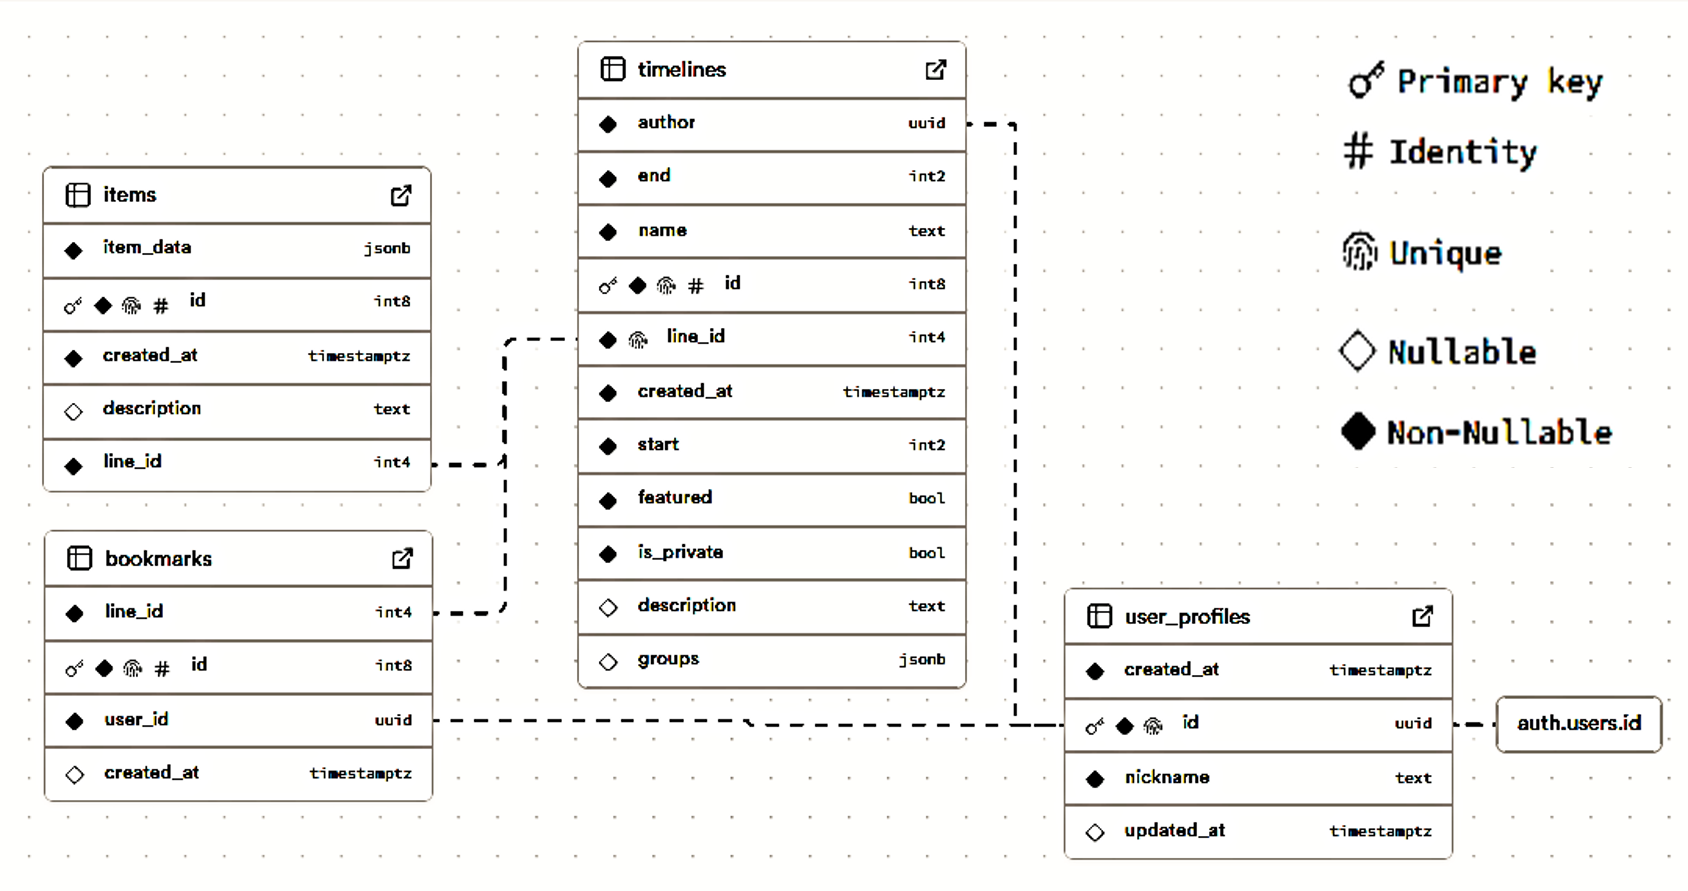
\includegraphics[width=1\linewidth]{Images/SupabaseStructure.png}
    \caption{Struktura tabulek z vizualizace v Supabase, legenda značek}
    \label{fig:Struktura tabulek}
\end{figure}

\subsubsection{Tabulka – timelines}
V centru celého systému stojí tabulka timelines, ve které jsou uložena všechna data, která se samotné časové osy týkají. Hlavními částmi jsou id, name – jméno dané časové osy, start a end, určující počátek a konec zobrazovaného období, line\_id, obsahující šestimístné číslo, které určuje odkaz na danou osu a zároveň slouží k propojení s dalšími tabulkami. \newpage
Featured je booleanová proměnná, která určuje, zda se daná osa zobrazí pro všechny uživatele na stránce v sekci „Vybrané“. Is\_private si nastavuje každý uživatel sám – určuje možnost návštěv autorovi osy jinými uživateli, více v sekci \ref{policies} \textit{Tabulková pravidla (policies)}. Uživatel si v časové ose také může nastavit jména jednotlivých řádků, což se ukládá ve formátu jsonb \cite{jsonb} do groups, a vlastní popis osy, který je uložen v description. 

\subsubsection{Tabulka – items}
Tabulka items zabezpečuje správné uložení jednotlivých událostí. Je propojená s tabulkou timelines pomocí cizího klíče line\_id. Obsahuje údaj o vytvoření a detailnější popis dané události, který má v databázi formát obyčejného textu, i když jsou v něm uloženy prvky v HTML syntaxi (\texttt{\textless h3\textgreater Nadpis \textless /h3\textgreater}).

Nejsložitější strukturou je pak určitě jsonb item\_data, který obsahuje všechny potřebné informace vyžadované knihovnou vue-timeline-chart ke správnému umístění na osu, viz ukázka \ref{item_data}.
Události jsem rozdělil na dva typy – kontextové a normální. Normální událost se skládá ze tří řádků: hlavní části, vedlejší a detailu (korespondující s označením řádků v kapitole \ref{Komponent časové osy}). Bohužel knihovna, kterou jsem využíval, neumožňuje přidat jednu událost na více řádků, proto jsem normální událost musel rozdělit do tří částí. Každý předmět má své unikátní id, začátek a konec, jméno, které se zobrazuje v časové ose, barvu nastavenou jako cssVariable, group označující řádek, kam bude umístěn, a poslední tag, podle kterého se sjednocují zmíněné tři části normální události. Kontextová událost je velice intuitivní, skládá se jen z jedné hlavní části a má všechny zmíněné proměnné stejné, jen tag je u ní vždy roven id.

\begin{lstlisting}[style=JavaScript, firstnumber = 1, caption={item\_data, Supabase items table}, label={item_data}]
{
  "id": 35,
  "end": -473385600000,
  "tag": 35,
  "name": "Osvicenstvi v literature",
  "group": 5,
  "start": -631152000000,
  "cssVariables": {
    "--item-background": "#073E5A"
  }
}
\end{lstlisting}

\subsubsection{Tabulka – user\_profile}
Tato tabulka je propojená se základní tabulkou auth.users.id a stará se o ukládání uživatelského nastavení. Protože jsem nechtěl, aby si jiní uživatelé mohli zobrazit váš e-mail, vytvořil jsem možnost nastavit si vlastní uživatelské jméno (nickname).  

\subsubsection{Tabulka – bookmarks}
Pro zlepšení uživatelského prostředí byla vytvořena tabulka bookmarks, která přidává uživateli funkci uložit si časové osy, které se mu líbily, a umožní mu k nim snadný přístup v sekci „Uložené“. Jsou v ní uložena ID časových os a UUID uživatelů.

\subsection{Tabulková pravidla (policies)}
\label{policies}
U všech svých tabulek mám zapnuté RLS neboli row-level security, které slouží k řízení přístupu k datům na úrovni jednotlivých řádků v tabulkách. Při použití RLS je důležité pečlivě nastavit příslušná pravidla (policies), která definují, kteří uživatelé nebo role mají jaká oprávnění pro čtení, vkládání, aktualizaci a mazání dat. Tato pravidla jsou definována pomocí SQL funkcí, které vracejí logickou hodnotu true nebo false v závislosti na kontextu aktuálního uživatele. V Supabase lze tato pravidla nastavovat přímo v uživatelském rozhraní. 

Například pro tabulku timeline mám nastavená pravidla: přidat novou osu může jen přihlášený uživatel, aktualizovat a mazat data může pouze autor dané časové osy. Pro zobrazení dat mám dvě pravidla – pokud je osa veřejná, nemusím kontrolovat nic. Pokud je ale osa soukromá, je nutné zjistit, zda je daný uživatel autorem, a na základě toho data buď zobrazit, nebo ne.


\begin{figure}[h]
    \centering
    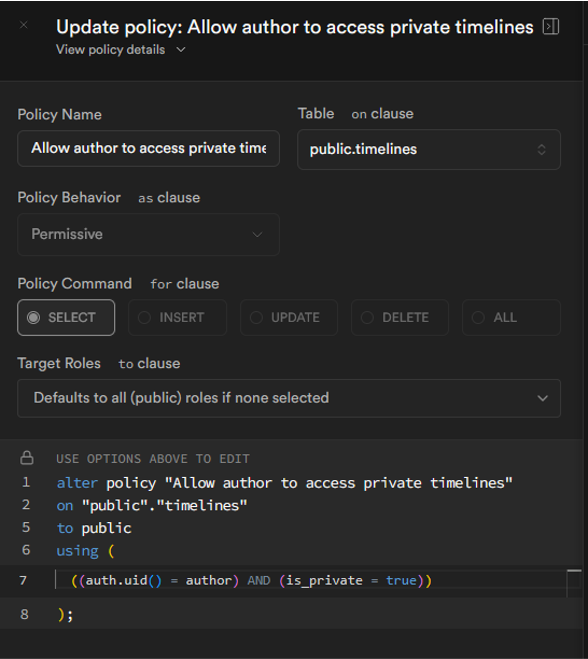
\includegraphics[width=0.45\linewidth]{Images/Policy_example.png}
    \caption{Ukázka nastavení pravidla tabulky v Supabase}
    \label{fig:Policy example}
\end{figure}

Zprvu jsem měl tuto ochranu jen na tabulku timelines, takže pokud by znal nepřihlášený uživatel id nějaké události v soukromé ose, mohl si ji zobrazit, i když k ose jako takové přístup neměl. Tento problém jsem samozřejmě opravil.

\newpage

\subsection{Práce s daty v databázi}
Díky ekosystému Nuxt je práce mezi programem a databází víceméně přímočará. Každá funkce v \textit{useSupabase.js} a \textit{supabaseItem.js} používá pro komunikaci s databází asynchronní funkci useSupabaseClient(), do které se zadají požadované SQL příkazy. Každá funkce má také návratovou hodnotu – ta může obsahovat samotná data při načítací funkci nebo odpověď databáze, buď o provedení, nebo o chybě, která nastala.

\subsection{Ukládání událostí}
Ukládání událostí je asi nejtěžší operace, při které záleží na různých parametrech, aby fungovala správně. Celý tento cyklus začíná v \textit{itemEditComp.vue}, kde se po zmáčknutí tlačítka „Uložit změny“ zavolá funkce saveChanges, která zkontroluje správnost zadaných roků, a pokud je vše správně, zavolá funkci handleItemUpdate z \textit{itemManipulation.js} se všemi parametry. Tato funkce se skládá ze tří částí: ukládání nově vytvořených částí, aktualizace již vytvořených a smazání nepotřebných událostí. Funkce se rozhoduje na základě parametrů od uživatele v porovnání s daty načtenými z databáze. Například pokud normální událost již měla v databázi uloženou hlavní a sekundární část a uživatel sekundární smazal, funkce zavolá \textit{updateItem}, aktualizuje hlavní část a sekundární smaže pomocí \textit{removeItem} z \textit{supabaseItem.js}. 

Při tvorbě nové části události je důležité podívat se na poslední použité ID a vytvořit další tak, aby se žádné neopakovalo. Dalším úskalím při tvorbě nové události je její uložení do správného řádku na základě parametrů contextType a isBottom, což řeší tato část kódu – ukázka \ref{groups}.      

\begin{lstlisting}[style=JavaScript, firstnumber = 154, caption={Handle update, itemManipulation.js}, label={groups}]
const mainGroup = contextType
  ? isBottom
    ? 8 : 1
  : isBottom
    ? 5 : 2;

  const secondaryGroup = isBottom ? 6 : 3;
  const detailGroup = isBottom ? 7 : 4;
\end{lstlisting}

Při tvorbě úplně nové události z postranního menu v \textit{SidebarComb.vue} používám stejnou funkci saveChanges, pouze je nastaven parametr pomocí query z přesměrování: \texttt{const creatingNew = ref(route.query.creatingNew === 'true');}.

\section{Řešení problémů}
V projektu jsem se několikrát potýkal s komplikacemi, ať už kvůli zbytečným chybám, nebo faktorům mimo moji kontrolu, a tak bych tady chtěl rozebrat pár problémů, se kterými jsem se setkal.

\subsection{Převádění času – Unixový čas}
\label{Převádění času - Unixový čas}

\subsubsection{Data před rokem 1970}
Na začátku projektu, když jsem se teprve učil pracovat s \textit{vue-timeline-chart}, jsem nastavil rozpětí let časové osy na 1950 až 2000. Po několika dnech od implementace jsem si ale všiml, že zobrazovaná část je pouze od roku 1970 do 2000. Bohužel jsem ve stejnou dobu pracoval na ovládání této osy, a tak jsem se snažil objevit chybu v posouvání zobrazené části a přibližování, která by mohla za useknutí dvaceti let. Asi týden jsem hledal tuto neexistující chybu, než jsem přišel na to, že rok 1950 je před začátkem unixového času. To znamená, že počet milisekund by měl být záporný.

\subsubsection{Data mezi lety 0 až 100}
Pro přeměnu milisekund na pro lidi příjemnější roky jsem využíval knihovní funkci \textit{Date.UTC(year, 0, 1)}. Tato funkce se zdála být více než dostačující pro převody let na milisekundy a naopak – až do chvíle, kdy jsem se snažil změnit roky před Kristem z formátu -50 až 50 na 50 BC až 50. Všiml jsem si totiž, že místo očekávaného roku 50 byl načten rok 1950. 

Pro kontrolu jsem používal online nástroj \textit{Epoch Converter} \cite{EpochConverter}, který ovšem nejspíše využívá stejnou metodu. Dlouho jsem přemýšlel, kde nastala chyba, než jsem otevřel oficiální dokumentaci \cite{Mozzila-UTC} a zjistil, že právě pro roky 0 až 100 jsou jejich hodnoty nastaveny jako roky 1900 až 2000. V dokumentaci jsem také hledal maximální a minimální hodnoty, které lze zadat do parametru roku, ale ty jsem nenašel. Metodou pokus-omyl jsem tedy dospěl k minimální hodnotě roku -271 820 a maximální 275 760. Tyto hodnoty ale nejsou plně podporovány komponentou časové osy, a tak jsou pro uživatelské zadávání povoleny hodnoty v rozmezí -12 000 až +12 000 let. 

Finální funkce pro převod z roku na milisekundy od epochy je uvedena v ukázce \ref{convertYearToMs} \cite{UTC-bugfix}.

\newpage
\begin{lstlisting}[style=JavaScript, firstnumber = 3, caption={itemManipulation.js, convertYearToMs}, label={convertYearToMs}]
export function convertYearToMs (year) {
  if (year >= 100 || year < 0) {
    return Date.UTC(year, 0, 1);
  } else {
    // For years before 100, we need to use a different approach
    const baseYear = year >= 0 ? 1900 : 2000;
    const yearDiff = Math.abs(year - baseYear);
    return -(-Date.UTC(baseYear, 0, 1) + (yearDiff * 31536000000));
  }
};
\end{lstlisting}

\subsubsection{Načtení dat roku 1970}
Poslední chyba, na kterou jsem narazil a která se vztahuje k převodům času, byl samotný rok 1970. Tento rok je totiž v milisekundách nula. Chyba nastala při načítání dat z databáze s nulovou milisekundovou hodnotou, kterou si můj program vyložil jako základní hodnotu nezadané položky – NaN (Not a Number) – a při převodu použil základní hodnotu 0 místo 1970. Oprava této chyby netrvala dlouho, stačilo přidat podmínku: pokud je hodnota NaN, nastav ji na 1970, viz [ukázka: \ref{loadItemData}].

\begin{lstlisting}[style=JavaScript, firstnumber = 110, caption={itemManipulation.js, loadItemData}, label={loadItemData}]
// ...
start: new Date(contextItem?.start || regularItem?.start).getFullYear() || 1970
// ...
\end{lstlisting}


\subsection{Předání informace nadřazenému souboru}
Jelikož ve svém projektu používám podmíněné renderování, které umožňuje zobrazit nebo skrýt různé komponenty, často mám nastavené základní rozvržení pozadí mimo danou komponentu. Někdy ale potřebuji předat informaci nadřazenému \textit{.vue} souboru, aby změnil stav nebo své vlastnosti. Přesně toto jsem potřeboval pro dynamické nastavení barvy z komponenty \textit{ItemEditComp.vue} na pozadí nadřazené stránky. Proto jsem použil funkci \textit{emit}.

Jako první musím nastavit konstantu \textit{emit} s daným jménem funkce, kterou chci provádět v nadřazeném komponentu. Poté nastavím pozorovatele (\textit{watcher}), který při zaznamenání změny hodnoty \textit{selectedColor} vyšle signál \textit{emit} s novou barvou.

Nadřazený komponent poslouchá \textit{event handler} \newline (@update-background="updateBackgroundColor"), a pokud takovou změnu objeví, provede se část kódu se jménem této změny. Funkce \textit{updateBackgroundColor} pak změní barvu pozadí v \texttt{div} díky reaktivnímu atributu \texttt{:style}.

\newpage
  \begin{lstlisting}[style=JavaScript, firstnumber = 1, caption={Update background; itemEditComp.vue, content.vue}, label={emits}]

// 1. Define emit
const emit = defineEmits(['update-background']);

// 2. Watch for color changes and emit them
watch(selectedColor, (newColor) => {
  emit('update-background', newColor);
});


////// Parent component ///////

<template>
    <div class="content\_box h-full w-full mx-10 px-4 md:px-6 relative "  
            :style="{ backgroundColor: backgroundColor }">
  <!-- Listen for emitted event -->
    <ItemEditComp v-if="inEdit" @update-background="updateBackgroundColor" />
    <ItemInfoComp v-if="!inEdit" @colorSelected="updateBackgroundColor" />
</template>

<script setup>
const backgroundColor = ref('#BAE6FD'); // Default color

// Handle the emitted event
function updateBackgroundColor(newColor) {
  backgroundColor.value = newColor;
}
</script>

\end{lstlisting}

Tento přístup zajišťuje konzistentní komunikaci mezi nadřazeným a podřazeným prvkem a umožňuje psát znovu použitelný kód. Ve zmíněném souboru je totiž ještě druhý \textit{event handler}, který místo na uživatelem vybranou barvu čeká na barvu načtenou z databáze skrze komponentu \textit{ItemInfoComp.vue}.

\section{Uživatelské rozhraní}
V této kapitole se pokusím vysvětlit, jak používat aplikaci, jak se ovládá a co se s ní dá dělat. Dále uvedu příklady mnou vytvořených časových os. 

\subsection{Navigace na stránce}
Stránka používá k navigaci horní lištu se záložkami jednotlivých sekcí stránek (tento prvek je uložen jako \textit{default.vue} ve složce \textit{layout}). Na menších zařízeních se místo záložek objeví rozklikávací menu pro výběr jednotlivých stránek.

\begin{figure}[h]
    \centering
    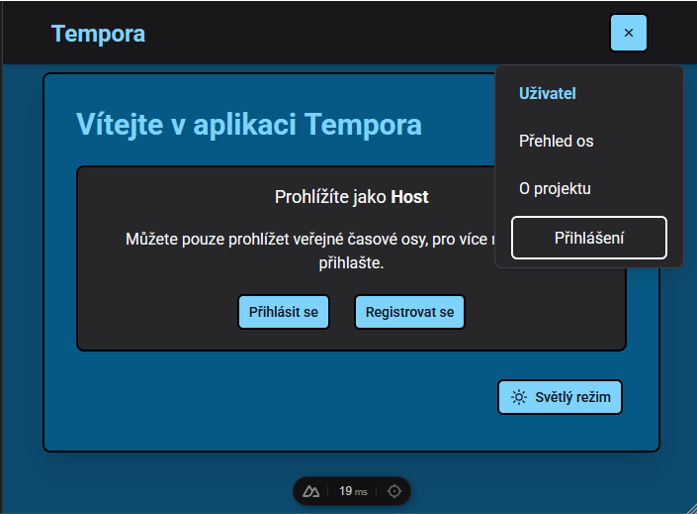
\includegraphics[width=0.6\linewidth]{Images/Mobile.png}
    \caption{Mobilní rozhraní ve tmavém režimu}
    \label{fig:mobile}
\end{figure}

\subsection{Tvorba osy}
Pokud je uživatel registrován a přihlášen, může vytvořit vlastní časovou osu. Nejprve se musí přesunout do sekce „Přehled os“, kde se nachází vybrané osy, osy vytvořené uživatelem a uložené osy, viz obrázek \ref{fig:LineHub}. V této sekci lze také vyhledávat osy podle jejich ID nebo celého odkazu. 

\begin{figure}[h]
    \centering
    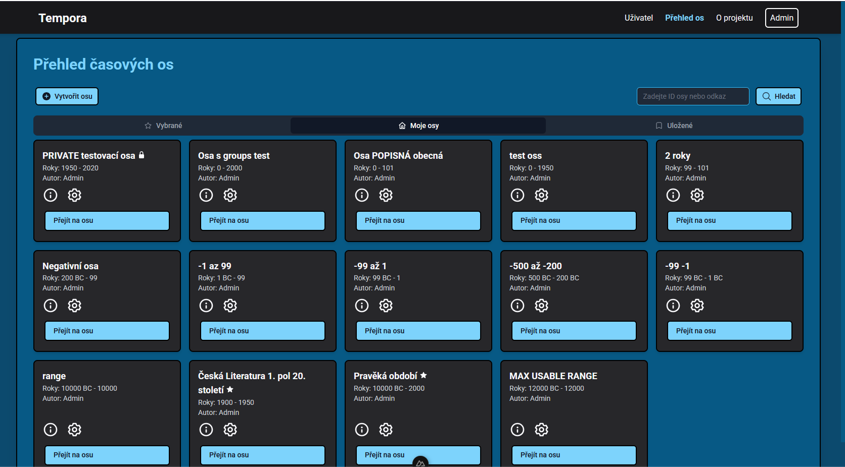
\includegraphics[width=0.8\linewidth]{Images/LineHub.png}
    \caption{Stránka Přehled os (tmavý režim)}
    \label{fig:LineHub}
\end{figure}

Po kliknutí na tlačítko „Vytvořit osu“ se otevře nová nabídka, kam uživatel zadává jméno časové osy, rok začátku a konce popisovaného období (pro zadání let před naším letopočtem se používá znak mínus před počtem let) a krátký popis dané osy, který může obsahovat například zdroje, odkud čerpal při tvorbě.

Na pravé straně je možnost pojmenovat jednotlivé řádky. Také lze nastavit osu jako soukromou, což znemožní komukoliv kromě autora si tuto osu zobrazit.

\begin{figure}[h]
    \centering
    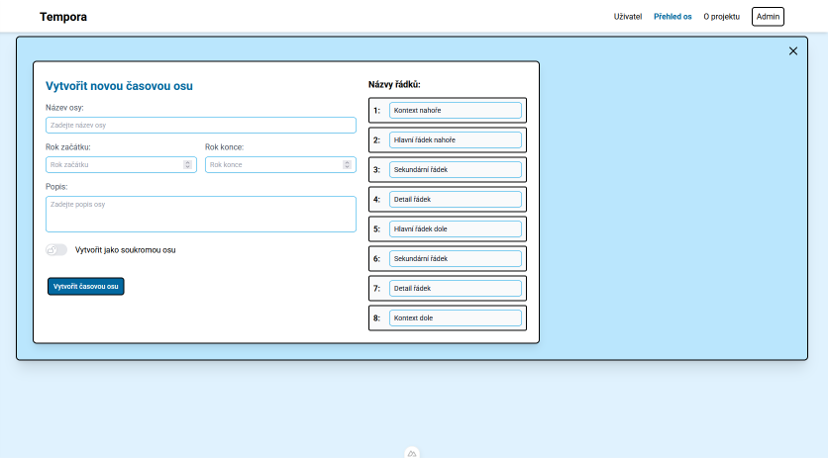
\includegraphics[width=0.8\linewidth]{Images/CreateNew.png}
    \caption{Tvorba nové osy (světlý režim)}
    \label{fig:CreateNew}
\end{figure}

\subsection{Ovládání osy}
Po vytvoření osy je uživatel přesunut přímo na stránku, kde se daná osa zobrazuje. Zde se nachází časová osa, uprostřed níž jsou uváděny letopočty. Pod osou je ovládací panel, pomocí kterého se osa posouvá, přibližuje nebo oddaluje. Nachází se zde také prvek, který ukazuje letopočet odpovídající pozici červené čáry a kurzoru umístěného na časové ose pro lepší orientaci. 

Klíčovou roli v ovládání má postranní lišta napravo, obsahující tlačítka: informace o ose, zapnutí editačního režimu, sdílení, nastavení, uložení, přidání nové události a přepnutí světlého/tmavého režimu.
\newpage

Na obrázku \ref{fig:AuthorTimeline} je zapnutý editační režim, což znamená, že po kliknutí na jednotlivé události je můžete upravovat. Zároveň se objeví nové tlačítko pro přidání události (více v sekci \ref{Úprava událostí} Úprava událostí). Tlačítko pro přepnutí časové osy do tmavého/světlého režimu funguje nezávisle na režimu celé aplikace a umožňuje uživateli zachovat jeho preferovaný režim, přičemž osu zobrazí v režimu, který se mu bude zdát příjemnější. 

Celou boční lištu lze také sbalit, aby nepřekážela. Pokud si prohlížíte osu, jejímž autorem nejste, uvidíte boční lištu tak, jak je zobrazena na obrázku \ref{fig:GuestTimeline}.


\begin{figure}[h]
    \centering
    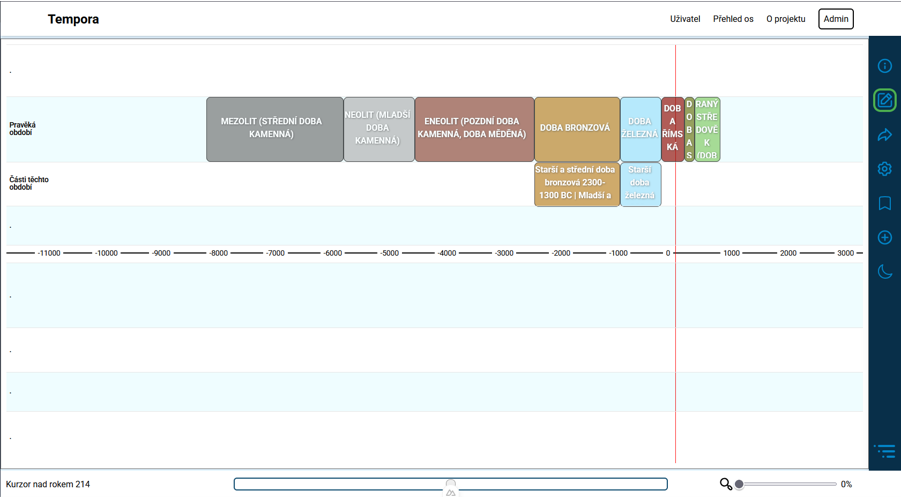
\includegraphics[width=0.8\linewidth]{Images/AuthorTimeline.png}
    \caption{Zobrazení postranní lišty - autor (světlí režim osy)}
    \label{fig:AuthorTimeline}
\end{figure}

\begin{figure}[h]
    \centering
    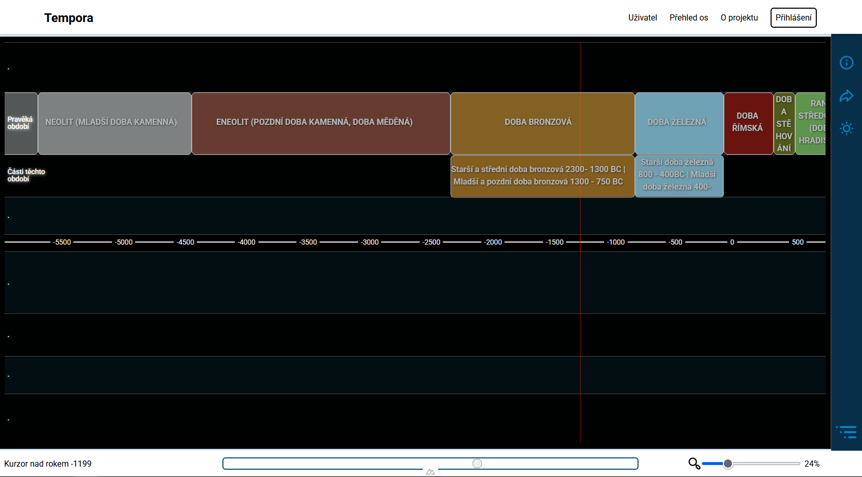
\includegraphics[width=0.8\linewidth]{Images/GuestTimeline.png}
    \caption{Zobrazení postranní lišty - návštěvník (tmavý režim osy)}
    \label{fig:GuestTimeline}
\end{figure}

\newpage

\subsection{Přidání a úprava události}
\label{Úprava událostí}
Pro přidání nové události musí být autor dané osy v editačním režimu a kliknout na tlačítko „Přidat událost“ (+), což ho přesměruje na URL nové události, kterou může začít upravovat, viz obrázek \ref{fig:NewItem}. 

V horní části si může vybrat, jestli chce vytvořit kontextovou nebo hlavní událost. Obě tyto části potřebují zadat roky trvání, aby se mohly na časovou osu umístit, a jejich zobrazované jméno, případně popis. Dále si také může vybrat, jakou barvu bude událost mít na časové ose – tato barva dynamicky mění okraj události. Pokud si uživatel zvolí hlavní událost, dostane možnost přidání vedlejší části a části detailu. Každá část umožňuje použít panel nástrojů pro editaci podrobností textu, odkazů, vzorců nebo zarovnání paragrafu. 

\begin{figure}[h]
    \centering
    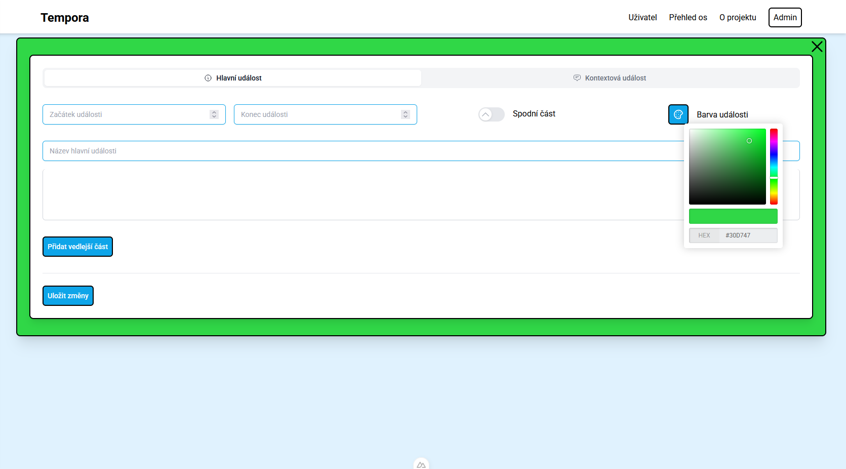
\includegraphics[width=0.8\linewidth]{Images/NewItem.png}
    \caption{Tvorba nové události}
    \label{fig:NewItem}
\end{figure}

Pokud chce uživatel upravit již vytvořenou událost, musí mít zapnutý editační režim a kliknout na událost na časové ose, kterou chce změnit. Otevře se mu stejné menu jako při tvorbě nové události, ale s načteným obsahem z databáze. Jedinou změnou je, že si nevybírá mezi hlavní a kontextovou událostí a může zahodit změny, které provedl, nebo smazat celou událost.  

\begin{figure}[h]
    \centering
    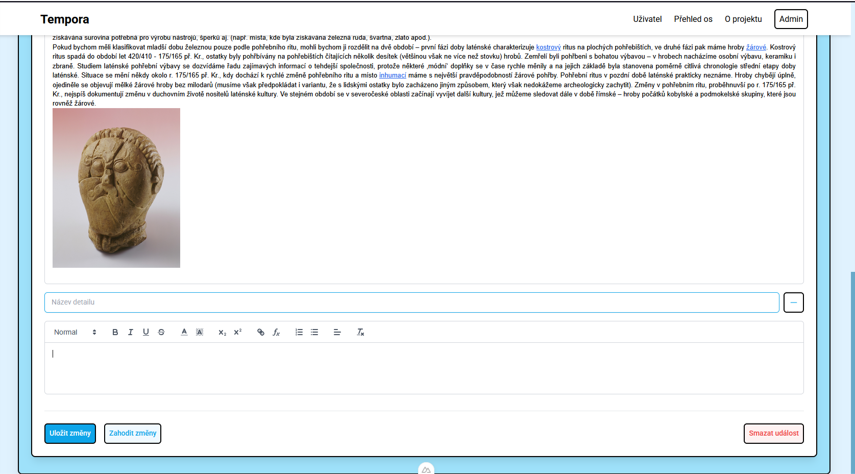
\includegraphics[width=0.8\linewidth]{Images/EditItem.png}
    \caption{Úprava již vytvořené události}
    \label{fig:EditItem}
\end{figure}


\subsection{Zobrazení události}
Pokud si chce uživatel prohlédnout podrobnosti o události, musí vypnout editační režim a kliknout na danou událost na časové ose. Poté se zobrazí stránka, na které jsou části rozděleny přesně podle toho, jak byly vytvořeny – s hlavním nadpisem a roky trvání. Pokud je vytvořeno více hlavních událostí v tomto řádku, objeví se nahoře také šipky pro přesměrování, ukazující, které období předcházelo a které následuje. 

\begin{figure}[h]
    \centering
    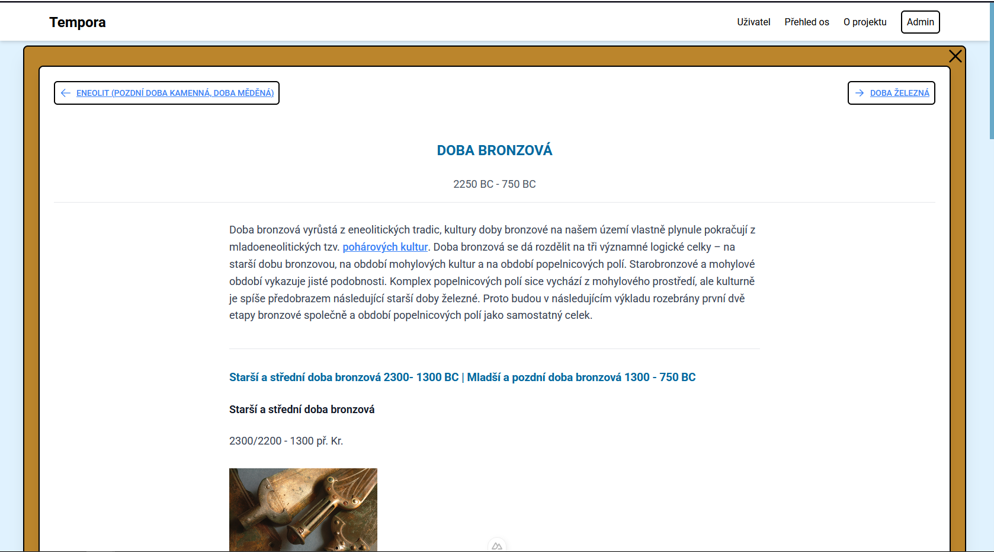
\includegraphics[width=0.8\linewidth]{Images/showItem.png}
    \caption{Ukázka zobrazení podrobností o události}
    \label{fig:showItem}
\end{figure}


\subsection{Vylepšení uživatelské zkušenosti}
Jedním z mých hlavních cílů bylo vytvořit uživatelsky příjemné a intuitivní prostředí. Proto jsem se již od začátku snažil tvořit prvky pro zpětnou vazbu – tlačítka změní barvu, když na ně najedete kurzorem, při načítání dat z databáze je vypsán aktuální stav toho, co se právě děje, a smazání údajů se nestane omylem díky potvrzovacímu dialogu. Celá webová aplikace podporuje světlý i tmavý režim (pomocí \textit{Tailwind} \texttt{dark:}), a časová osa má svůj vlastní přepínač, aby se zabránilo špatně vypadajícím barvám v jednom z režimů. 

Aplikace často využívá ikony z knihovny \textit{Iconify} \cite{Icons-pack} pro zlepšení přehlednosti. Pokud jsou tyto ikony použity místo tlačítek, vždy se při najetí kurzorem zobrazí popisek vysvětlující jejich funkci. \newpage Uživatel si při tvorbě událostí a podrobností může sám zvolit jednotlivé barvy událostí díky komponentě \cite{ColorPicker-module}, a při tvorbě textu může využít prvky jako odrážky, tučné písmo, podtržení, vložení odkazu a mnoho dalších díky „HTML RichText“ z knihovny \textit{Quill} \cite{Quill-lib}. V celém projektu používám font \textit{Google Roboto} \cite{Roboto}.

Aplikace by měla být plně responzivní a použitelná i na mobilu díky \textit{Tailwind} prefixům \texttt{md:}, \texttt{lg:}, i když hlavním záměrem byla verze pro počítač.

\subsection{Ukázka hotových os}
Pro tento projekt jsem vytvořil dvě ukázkové osy. Pro ukázku širokého rozpětí osy „Pravěká období“, která začíná 8000 let před naším letopočtem a končí rokem 1000, a pro ukázku použití kontextu a událostí v kratší časové době jsem vytvořil osu s názvem „Česká literatura první poloviny dvacátého století“. 

Při tvorbě ukázkových časových os jsem použil stránky Národního muzea \cite{archeologie-pravek} a Wikipedie \cite{literatura-wiki}. Tyto časové osy nemusí být stoprocentně přesné a slouží pouze k demonstraci použití mé webové aplikace.


\begin{figure}[h]
    \centering
    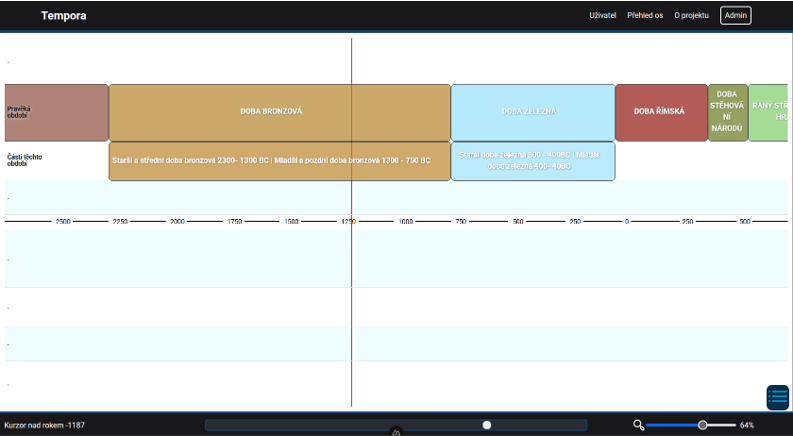
\includegraphics[width=1\linewidth]{Images/Detail-pravěk.png}
    \caption{Ukázka zobrazení přiblížené Pravěké osy }
    \label{fig:Detail-pravěk}
\end{figure}

\begin{figure}[h]
    \centering
    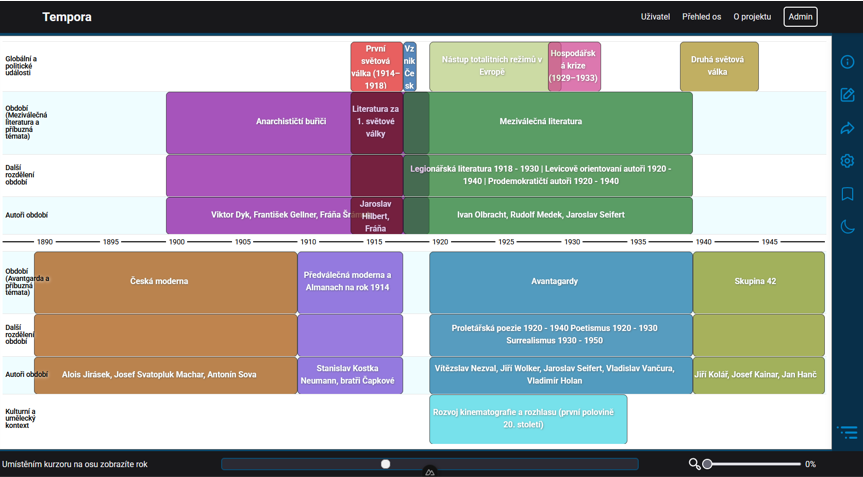
\includegraphics[width=1\linewidth]{Images/lit.png}
    \caption{Ukázka oddálené časové osy Literatura 20. století}
    \label{fig:lit}
\end{figure}

\begin{figure}[h]
    \centering
    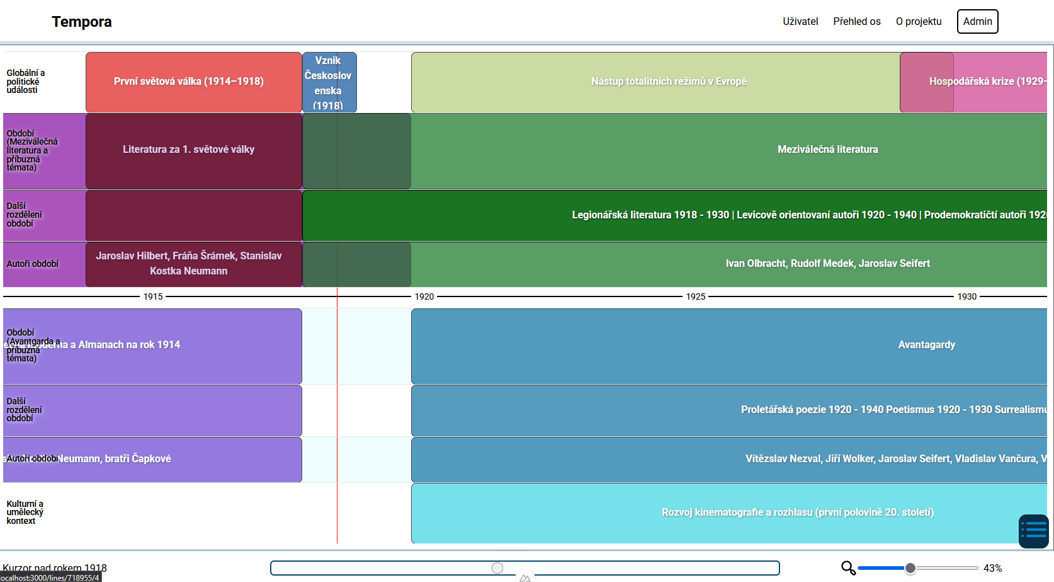
\includegraphics[width=1\linewidth]{Images/Detail-lit.png}
    \caption{Ukázka přiblížené časové osy Literatura 20. století}
    \label{fig:Detail-lit}
\end{figure}

\begin{figure}[h]
    \centering
    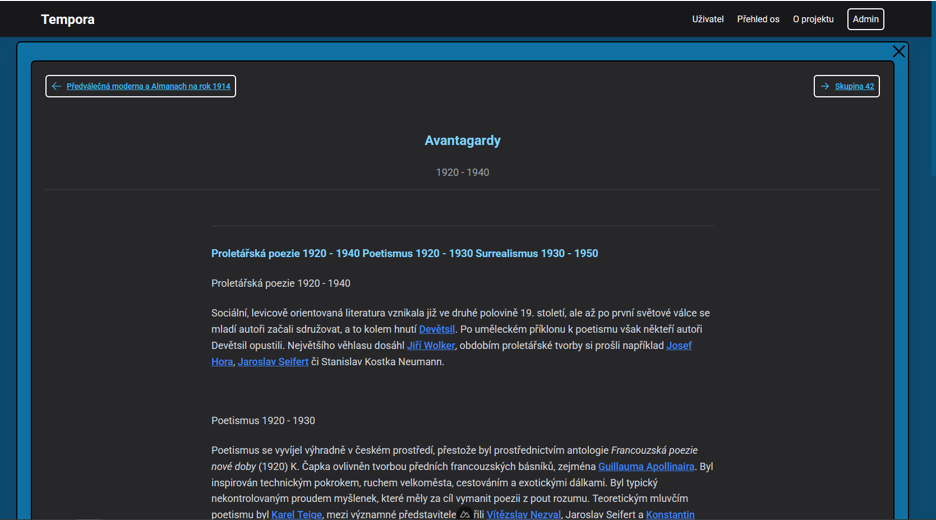
\includegraphics[width=1\linewidth]{Images/podrobnosti-lit.png}
    \caption{Ukázka zobrazení podrobností Avantgardy (tmavý režim)}
    \label{fig:podrobnosti-lit}
\end{figure}

\begin{figure}[h]
    \centering
    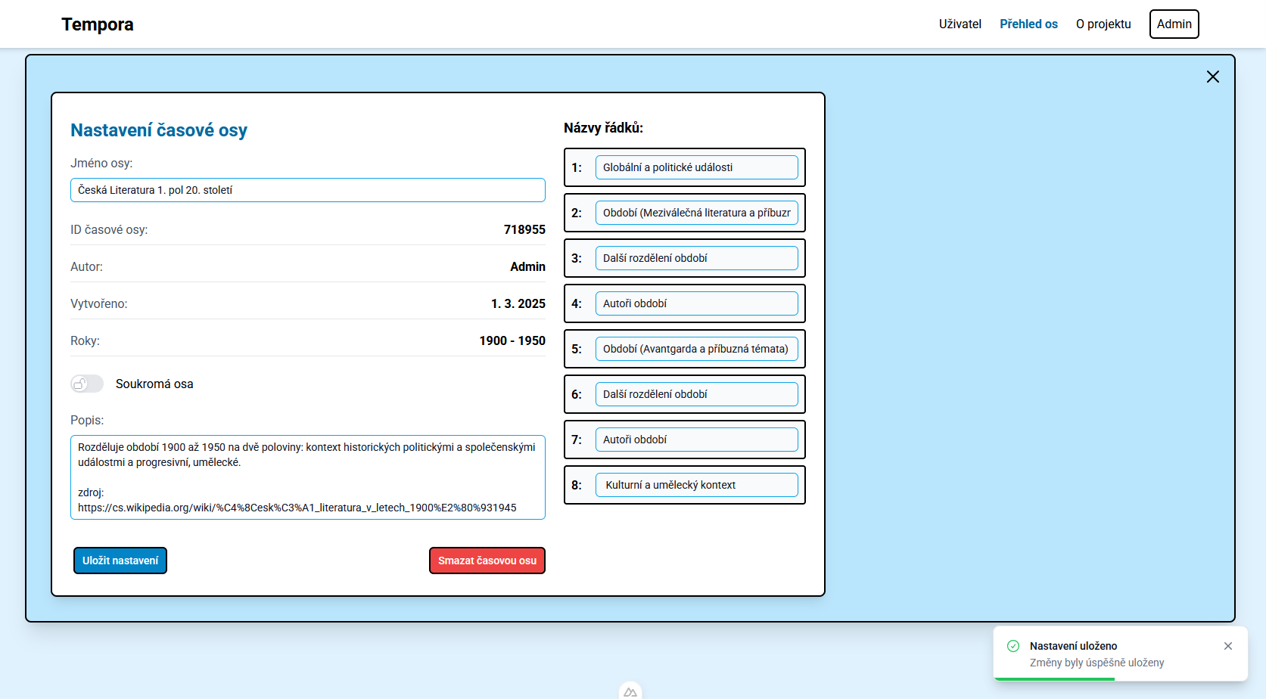
\includegraphics[width=1\linewidth]{Images/Settings.png}
    \caption{Ukázka možností nastavení časové osy s notifikací o uložení}
    \label{fig:Settings}
\end{figure}
\section{Aplikace ve výuce a didaktický přínos}

\subsection{Výukový cíl}
Primárním cílem této pomůcky je pomoci studentům a učitelům přehledně rozdělit daná témata v určitém období a přidat k nim potřebný kontext, případně srovnání s jinými událostmi. K jednotlivým událostem také patří jejich popis a další informace, které jsou vhodné i pro učení látky jako takové.

\subsection{Didaktické zařazení}
Tato aplikace nabízí možnost využití napříč různými odvětvími. Mezi hlavní patří dějepis, literatura, hudební či výtvarné umění v rámci historie. V těchto předmětech by Tempora mohla být použita jako jedna z hlavních výukových pomůcek. Své uplatnění by ale mohla najít i mimo humanitní vědy, a to ve více technických předmětech, jako je fyzika, chemie, biologie a další, kde by pomohla přiblížit historický kontext objevů a důležitých vynálezů. Zde by mohla sloužit pouze jako vedlejší pomůcka studentům k srovnání jednotlivých letopočtů a dat daných událostí. Tato aplikace je vhodná pro použití od druhého stupně základní školy až do vyšších ročníků středních škol a gymnázií.



\subsection{Využití ve výuce}
Využití v samotných hodinách může mít různou formu. Učitel si může připravit osu na dané téma a ukazovat na ní jednotlivá období. Odkaz na tuto osu pak může pomocí například Google Classroom nebo Microsoft Teams nasdílet do učebny pro samostatné studium. Další možností je zadat nějaké téma a nechat ho zpracovat studenty v hodině, následně jej prezentovat před třídou. Učitel může také zadat tvorbu osy jako dobrovolný či povinný domácí úkol.



\subsection{Dotazník pro studenty}
\label{Dotazník}

Abych zjistil, co si o aplikaci myslí studenti, nechal jsem otestovat svůj projekt několika spolužáky, kteří mi následně vyplnili dotazník. Ten bych zde chtěl rozebrat.

\subsubsection{Testování aplikace}
Aplikaci jsem nasadil na vlastní server a pomocí služby Ngrok\cite{ngrok} sdílel vygenerovanou zabezpečenou URL. Tento způsob jsem zvolil pouze pro testování a v rámci rychlého sdílení projektu. Pokud by se projekt měl aplikovat ve velkém měřítku, je samozřejmě možné pomocí Dockeru aplikaci nasadit na placený server s vlastní doménou.


\subsubsection{Výsledky průzkumu}
V dotazníku vytvořeném v Google Forms jsem se ptal na různé aspekty aplikace – od zkušeností s používáním, přes nalezené problémy až po její využití ve výuce.
Pro mě nejdůležitějším tématem byla přehlednost a jednoduchost aplikace, na což jsem se zeptal v otázkách 1 a 2 (obrázek \ref{fig:graf12}).

\begin{figure}[h]
\begin{minipage}[]{0.5\linewidth}
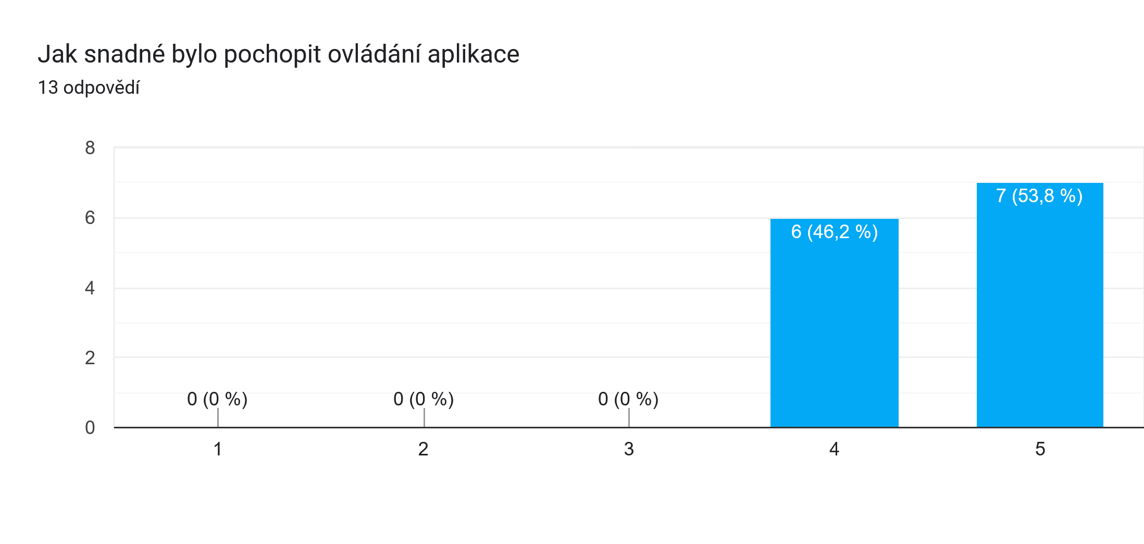
\includegraphics[width=\linewidth]{Images/graf1.png}
\end{minipage}
\hfill
\begin{minipage}[]{0.5\linewidth}
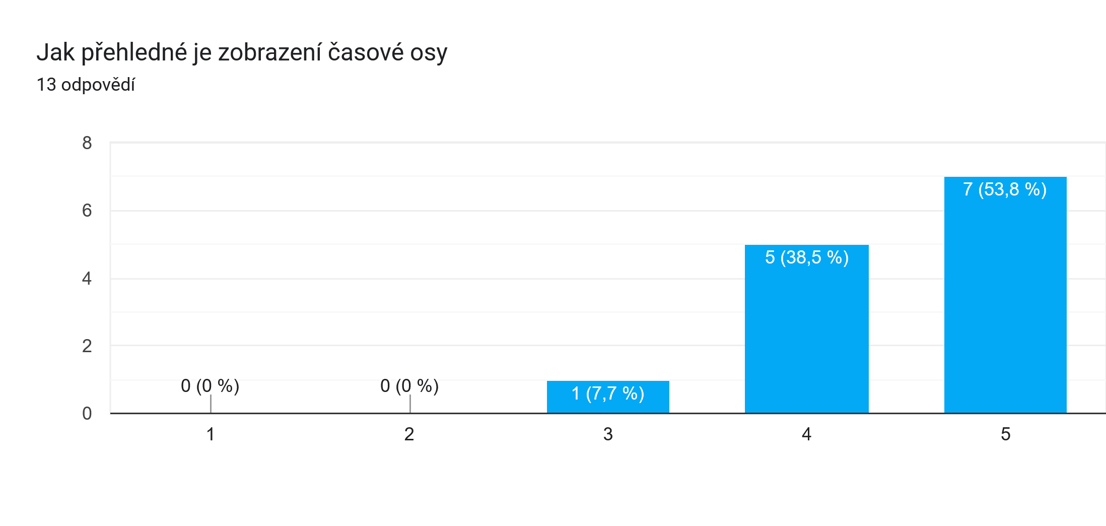
\includegraphics[width=\linewidth]{Images/graf2.png}
\end{minipage}%
\caption{Grafy první a druhé otázky dotazníku}
\label{fig:graf12}
\end{figure}

Z grafu jednoznačně vyplývá, že můj záměr byl úspěšný – respondenti označili aplikaci jako velmi snadnou a přehlednou. Stejný závěr měla i otázka 3: Jak užitečné jsou vizuální prvky (barvy, rozložení, styl), kde byly nejčastěji zvoleny možnosti 4 nebo 5 (5 = velmi užitečné).

\begin{figure}[h]
    \centering
    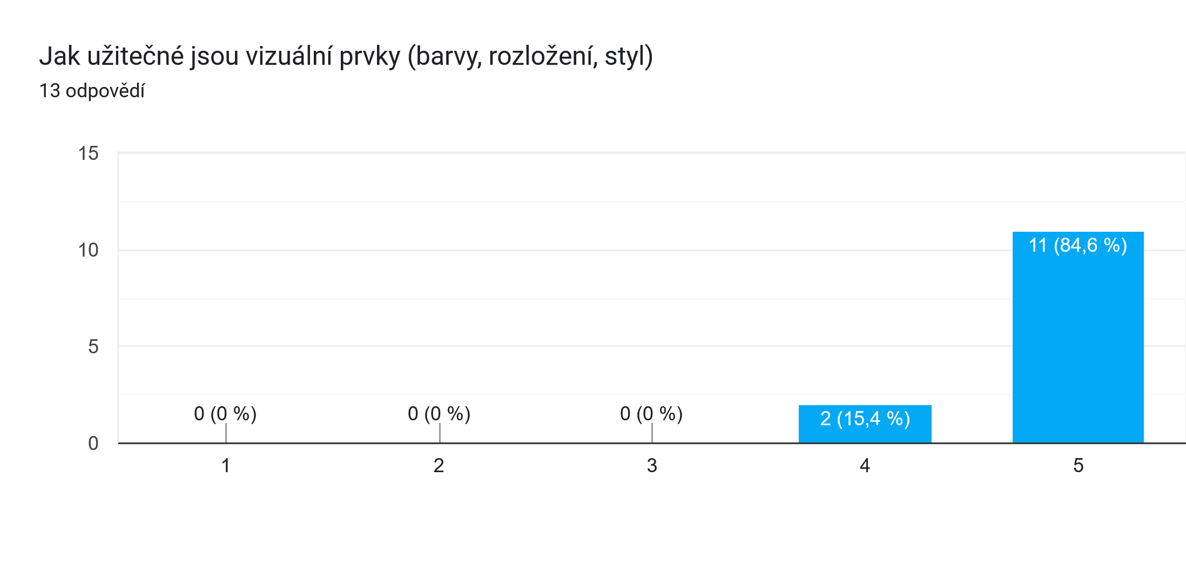
\includegraphics[width=0.8\linewidth]{Images/graf3.png}
    \caption{Graf 3. otázky dotazníku}
    \label{fig:graf3}
\end{figure}

\newpage
Čtvrtá otázka se věnovala využití aplikace ve výuce s historickým kontextem. S velkou převahou vede odpověď: Používal bych tuto aplikaci v kombinaci s jinými zdroji, což znamená, že aplikace je užitečná, ale nenahrazuje kompletně ostatní výukové prostředky.

\begin{figure}[h]
    \centering
    
\includegraphics[width=0.8\linewidth]{Images/graf4.png}
    \caption{Graf 4. otázky dotazníku}
    \label{fig:graf4}
\end{figure}

V otázce číslo pět jsem se respondentů zeptal, jak si představují využití aplikace ve výuce. Tato otázka umožňovala více vybraných možností (viz obrázek \ref{fig:graf5}).

\begin{figure}[h]
    \centering
    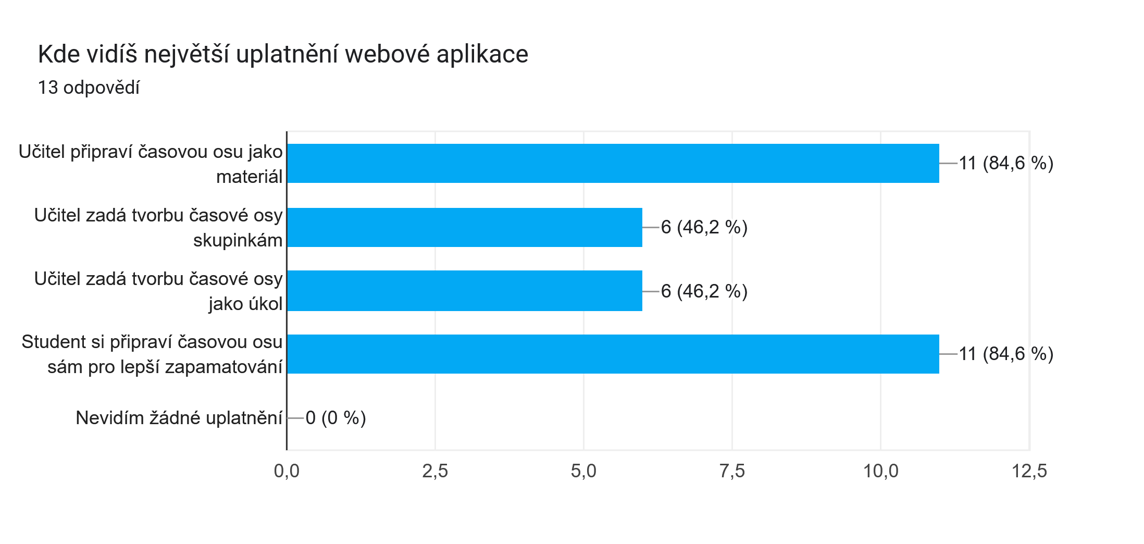
\includegraphics[width=0.8\linewidth]{Images/graf5.png}
    \caption{Graf 5. otázky dotazníku}
    \label{fig:graf5}
\end{figure}


Na prvním místě se shodným počtem hlasů umístily odpovědi 1 a 4.
O zhruba polovinu hlasů méně získaly odpovědi 2 a 3.
Tento výsledek ukazuje, že studenti více preferují použití osy samostatně před skupinovou prací a dávají přednost studiu z vlastní iniciativy nebo výuce z učitelovy časové osy před povinným úkolem.

V poslední části dotazníku jsem se ptal na zpětnou vazbu a možná vylepšení, která respondenty napadla.

Jedna z odpovědí si stěžovala na zpočátku těžce pochopitelné ovládání.
Tento problém by se dal vyřešit přidáním stránky s návodem nebo navedením nového uživatele pomocí vysvětlivek, jak časová osa funguje.
Další dotaz se týkal možnosti zadání přesného data. Tato funkce nebyla přidána kvůli zjednodušení databázového systému a proto, že osa má sloužit primárně k zobrazování delších období. Pokud však uživatel chce zdůraznit určité datum, může jej uvést do názvu období.
\section{Možná budoucí vylepšení}
Jako téměř jakýkoliv projekt ani tento není naprosto perfektní a vždy je možné něco zlepšovat. Proto bych tuto kapitolu chtěl věnovat možným budoucím vylepšením, která nejsou implementována, ale mohla by projekt posunout dále. Nebudu zde uvádět již zmíněné problémy v části \ref{Dotazník} \textit{Dotazník pro studenty}.

\subsection{Uživatelská vylepšení}

\subsubsection{Kategorie}
Jedna z věcí, která je v mé stávající verzi obtížná, je možnost objevovat nové osy jiných uživatelů. Nyní je sice možné sdílet osy pomocí odkazu nebo ID, ale při nasazení aplikace pro veřejnost nastává problém s tím, jak tyto osy efektivně vyhledávat podle toho, co mě zajímá nebo co se mi líbí. Nebylo by tedy špatné implementovat ověřený systém kategorií nebo hashtagů s různými tématy, podle kterých by se daly jednotlivé osy vyhledávat. 

\subsubsection{Hodnocení}
Dále, pokud bych přidal vyhledávání veřejných os, nabízí se vytvořit uživatelské hodnocení, které by mohlo fungovat podobně jako např. na platformě \href{https://www.reddit.com/}{Reddit}, kde uživatelé hodnotí buď kladně („up-vote“), nebo záporně („down-vote“).

\subsubsection{Admin role}
Zlepšit by se dala i funkce vybraných os. Tuto funkci jsem přidal hlavně z důvodu zobrazení alespoň nějakého úvodního obsahu pro nepřihlášené uživatele. Tento koncept by se ale mohl posunout dále a vytvořit roli admina, který může ocenit správně udělané časové osy, jež mají velké množství kladných bodů, a napevno je umístit do sekce „Vybrané“ přímo z UI aplikace, a ne přes editaci tabulky skrze SQL příkaz.

\subsection{Další návrhy}

\subsubsection{Překlad}
Když jsem s projektem začínal a ještě nevěděl, jak se co bude jmenovat, náhodně jsem používal  česko-anglické názvy. Později, když už jsem získal představu, jak chci, aby aplikace vypadala, jsem si musel vybrat, jestli ji nechat celou v angličtině, nebo celou v češtině. Zvolil jsem češtinu, ale nebylo by špatné, pokud by se aplikace více rozšířila, nechat uživatele vybrat si svůj jazyk.

\subsubsection{Shrnutí období}
Zajímavá funkce, která mě napadla, by bylo shrnutí roku. Tato funkce by umožnila uživateli vybrat nějaké období a poté by z dat vybraných os vrátila vše, co se v daném roce stalo. Tato možnost je ale pouze návrh, protože by velice záleželo na implementaci, např. z jakých os by se data brala, kolik dat vzít nebo jak zajistit, že uživatel dostane relevantní informace.

\section{Závěr}

Když jsem s prací začínal, nevěděl jsem o frameworku Nuxt téměř nic, ale postupnou prací na projektu jsem se mnoho naučil. Kupříkladu, jak pracovat s databází, vytvořit přehlednou strukturu projektu nebo jak vytvářet uživatelsky příjemné prostředí.

Důležité při projektu tohoto rozsahu bylo dobře si rozdělit čas, pracovat na projektu průběžně a organizovat plán, jak implementovat jednotlivé funkce, sepisovat si nápady a zaznamenat si, pokud nějaká část aplikace nefunguje správně.

Povedlo se mi tedy vytvořit interaktivní webovou aplikaci pro vlastní tvorbu a prohlížení časových os, která dokáže přehledně vizualizovat daná období a zobrazit o nich podrobnější informace, umožnit porovnání tematicky odlišných událostí v jedné době nebo přidat potřebný historický kontext. 

Práce tedy splnila mé očekávání, i když je vždy co dodělávat, a jak jsem zmínil, existují další nápady na nové funkce a vylepšení, na kterých bych určitě chtěl pracovat i v budoucnu.


\section{Použité zdroje}
\printbibliography[heading=none]


\newpage
\mbox{}
\addcontentsline{toc}{section}{\listfigurename}
\listoffigures

\mbox{}
\addcontentsline{toc}{section}{\lstlistlistingname}
\lstlistoflistings

\end{document}
